% Crank-001 readout deck --- the first measured reverse-diffusion step over the
% ratio spec corpus. Built via rules_tectonic (//deck:crank001). The hero graph
% figures (figures/crystal.pdf, collapse_before.pdf, collapse_after.pdf) are
% rendered from the authored //graph .dot sources by the host-`dot` bridge in
% BUILD.bazel; the native data figures are pgfplots/TikZ. Companion to the
% crystallization whitepaper (//paper:crystallization), RFC-001, RFC-001b.
\documentclass[aspectratio=169,11pt]{beamer}

\usepackage[T1]{fontenc}
\usepackage{lmodern}
\usepackage{booktabs}
\usepackage{array}
\usepackage{pifont}
\usepackage{graphicx}
\usepackage{tikz}
\usepackage{pgfplots}
\pgfplotsset{compat=1.18}
\usetikzlibrary{arrows.meta,positioning,calc,shapes.geometric}

% ---- ratio brand palette ----
\definecolor{ratioInk}{HTML}{3A2A1C}
\definecolor{ratioBrown}{HTML}{6E4F34}
\definecolor{ratioTan}{HTML}{B98E5E}
\definecolor{ratioSand}{HTML}{D9C19A}
\definecolor{ratioCream}{HTML}{F4EEDD}
\definecolor{openGreen}{HTML}{2F6B2F}
\definecolor{paywallRed}{HTML}{9B2C2C}

% ---- theme ----
\usetheme{default}
\setbeamertemplate{navigation symbols}{}
\setbeamercolor{normal text}{fg=ratioInk}
\setbeamercolor{structure}{fg=ratioBrown}
\setbeamercolor{title}{fg=ratioInk}
\setbeamercolor{frametitle}{fg=ratioCream,bg=ratioBrown}
\setbeamercolor{itemize item}{fg=ratioTan}
\setbeamercolor{itemize subitem}{fg=ratioTan}
\setbeamercolor{block title}{fg=ratioCream,bg=ratioBrown}
\setbeamercolor{block body}{fg=ratioInk,bg=ratioCream}
\setbeamerfont{frametitle}{series=\bfseries}
\setbeamerfont{title}{series=\bfseries,size=\LARGE}
\setbeamertemplate{itemize item}{\ding{228}}
\setbeamertemplate{itemize subitem}{\ding{229}}

% A slim brown frametitle bar.
\setbeamertemplate{frametitle}{%
  \nointerlineskip%
  \begin{beamercolorbox}[wd=\paperwidth,ht=2.6ex,dp=1.1ex,leftskip=0.5em,rightskip=0.5em]{frametitle}%
    \usebeamerfont{frametitle}\insertframetitle%
  \end{beamercolorbox}%
}

% Footline: wordmark + short title + page.
\setbeamertemplate{footline}{%
  \leavevmode\hbox{%
    \begin{beamercolorbox}[wd=.28\paperwidth,ht=2.4ex,dp=1ex,leftskip=0.6em]{frametitle}%
      \textbf{ratio}\,\textbar\,spec%
    \end{beamercolorbox}%
    \begin{beamercolorbox}[wd=.55\paperwidth,ht=2.4ex,dp=1ex,leftskip=0.6em]{block body}%
      \scriptsize Crank-001 readout%
    \end{beamercolorbox}%
    \begin{beamercolorbox}[wd=.17\paperwidth,ht=2.4ex,dp=1ex,rightskip=0.6em]{block body}%
      \scriptsize\hfill\insertframenumber\,/\,\inserttotalframenumber\;%
    \end{beamercolorbox}%
  }%
}

% Big-number stat tile.
\newcommand{\stat}[3]{%
  \begin{beamercolorbox}[wd=#1,ht=10ex,dp=1ex,center]{block body}%
    \vskip2pt{\color{ratioBrown}\textbf{\LARGE #2}}\\[2pt]{\scriptsize #3}\vskip2pt%
  \end{beamercolorbox}%
}

\title{Crank-001}
\subtitle{The first measured reverse-diffusion step over the ratio spec corpus}
\date{2026-06-26}

\begin{document}

% ---------------------------------------------------------------- title
{%
\setbeamertemplate{footline}{}
\begin{frame}[plain]
  \vfill
  \begin{center}
    {\color{ratioBrown}\rule{0.5\textwidth}{1.5pt}}\\[1.2em]
    {\usebeamerfont{title}\inserttitle}\\[0.6em]
    {\large\color{ratioInk}\insertsubtitle}\\[1.0em]
    {\color{ratioBrown}\rule{0.5\textwidth}{1.5pt}}\\[1.4em]
    {\footnotesize\color{ratioInk}Result log\, \textbar\, companion to the crystallization whitepaper, RFC-001, RFC-001b\, \textbar\, \insertdate}
  \end{center}
  \vfill
\end{frame}
}

% ---------------------------------------------------------------- frame: frame
\begin{frame}{The frame: refinement is annealed descent of an energy}
  \begin{columns}[T]
    \begin{column}{0.56\textwidth}
      \begin{itemize}
        \item A spec corpus is a \textbf{typed graph} of claims and edges.
        \item ``Rough'' = high energy: redundant, contradictory, dangling, under-specified.
        \item \textbf{Refinement} = lower the energy by a \emph{predict $\to$ project} step, annealing the temperature toward zero.
        \item One such step is a \textbf{crank}. This deck is the readout of the first one.
      \end{itemize}
      \vskip0.6em
      \begin{block}{The spec energy}
        \[
          E(G)=\underbrace{w_1R+w_2C+w_3D+w_4U}_{\text{costs: drive down}}\;-\;\underbrace{w_5L+w_6S}_{\text{structure: drive up}}
        \]
      \end{block}
    \end{column}
    \begin{column}{0.42\textwidth}
      \centering
      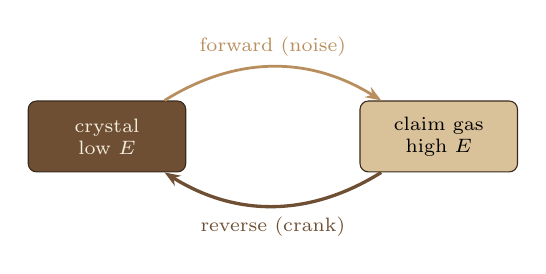
\begin{tikzpicture}[font=\scriptsize,>={Stealth[length=2mm]}]
        \node[draw=ratioInk,fill=ratioBrown,text=ratioCream,rounded corners=3pt,
              minimum width=20mm,minimum height=9mm,align=center] (cr) {crystal\\\scriptsize low $E$};
        \node[draw=ratioInk,fill=ratioSand,rounded corners=3pt,
              minimum width=20mm,minimum height=9mm,align=center,right=22mm of cr] (gas) {claim gas\\\scriptsize high $E$};
        \draw[->,ratioTan,line width=1pt] (cr) to[bend left=32] node[above,font=\scriptsize\color{ratioInk}]{forward (noise)} (gas);
        \draw[->,ratioBrown,line width=1.2pt] (gas) to[bend left=32] node[below,font=\scriptsize\color{ratioInk}]{reverse (crank)} (cr);
      \end{tikzpicture}
      \vskip1.2em
      {\scriptsize The crank runs the \emph{reverse} arrow: from rough corpus toward a compact, strongly-linked crystal.}
    \end{column}
  \end{columns}
\end{frame}

% ---------------------------------------------------------------- frame: E(G0)
\begin{frame}{What one crank measured: \texorpdfstring{$E(G_0)$}{E(G0)}}
  \begin{columns}[T]
    \begin{column}{0.54\textwidth}
      {\footnotesize The four \textbf{cost} terms (drive down):}
      \vskip2pt
      % Cost terms of E(G_0) measured by crank-001 — the four we want to drive down.
% (Structure terms L=64 edges, S=7 templates are shown as stat tiles on the
% slide; they live on a different scale and we want them to rise, not fall.)
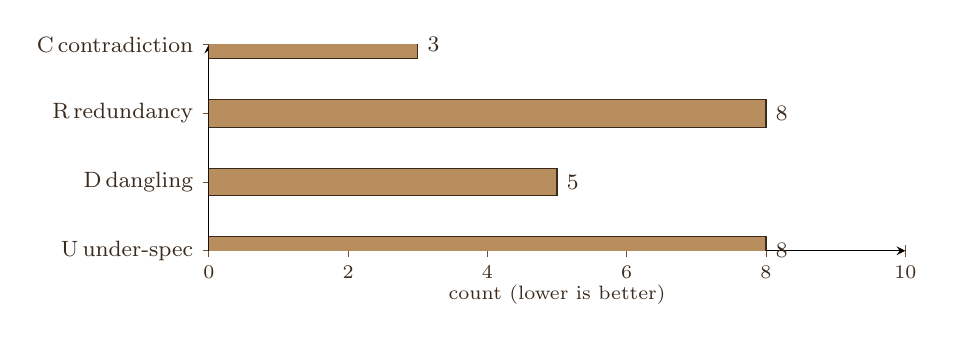
\begin{tikzpicture}
\begin{axis}[
  xbar,
  width=0.86\linewidth, height=4.2cm,
  bar width=10pt,
  xmin=0, xmax=10,
  enlarge y limits=0.28,
  axis lines=left,
  xlabel={count (lower is better)},
  every axis x label/.style={at={(axis description cs:0.5,-0.12)},anchor=north,
                             font=\scriptsize\color{ratioInk}},
  symbolic y coords={U\,under-spec,D\,dangling,R\,redundancy,C\,contradiction},
  ytick=data,
  yticklabel style={font=\footnotesize\color{ratioInk}},
  xtick={0,2,4,6,8,10},
  xticklabel style={font=\scriptsize\color{ratioInk}},
  nodes near coords,
  nodes near coords style={font=\footnotesize\bfseries\color{ratioInk}},
  every node near coord/.append style={anchor=west},
  tick style={color=ratioBrown},
]
\addplot[draw=ratioInk, fill=ratioTan] coordinates {
  (8,U\,under-spec)
  (5,D\,dangling)
  (8,R\,redundancy)
  (3,C\,contradiction)
};
\end{axis}
\end{tikzpicture}

    \end{column}
    \begin{column}{0.44\textwidth}
      {\footnotesize The two \textbf{structure} terms (drive up):}
      \vskip4pt
      \hbox to \linewidth{\stat{0.46\linewidth}{64}{typed edges $L$ over 73 claims; 3 hubs}\hfill\stat{0.46\linewidth}{7}{motif templates $S$ cover all 16 specs}}
      \vskip0.8em
      \begin{block}{Dominant signal}
        \footnotesize Highly \textbf{symmetric} and \textbf{redundant} (big recoverable $S$, big $R$); one important contradiction ($C$); a frontier ($U$) that is mostly groundable from \textbf{open} sources.
      \end{block}
    \end{column}
  \end{columns}
\end{frame}

% ---------------------------------------------------------------- frame: HERO crystal
\begin{frame}{The corpus is a near-star around conservation}
  \begin{columns}[c]
    \begin{column}{0.66\textwidth}
      \centering
      \includegraphics[height=0.78\textheight]{../graph/crystal_pdf}
    \end{column}
    \begin{column}{0.33\textwidth}
      {\footnotesize
      \textbf{3 hubs} carry the graph:
      \begin{itemize}\setlength\itemsep{2pt}
        \item \texttt{core:2} --- conservation (net vector $=0$)
        \item \texttt{core:12} --- the single write-door
        \item \texttt{pa:3} --- read projections
      \end{itemize}
      \vskip4pt
      \textbf{7 motif templates} (tan) ring the hubs; \textbf{component instances} (cream) at the rim.
      \vskip4pt
      \textbf{Frontier standards} attach as notes:\\
      {\color{openGreen}\ding{108}} open\quad{\color{paywallRed}\ding{108}} paywalled.
      }
    \end{column}
  \end{columns}
\end{frame}

% ---------------------------------------------------------------- frame: collapse
\begin{frame}{The symmetry collapse: 16 specs are one orbit}
  \begin{columns}[c]
    \begin{column}{0.47\textwidth}
      \centering
      \includegraphics[width=\linewidth,height=0.60\textheight,keepaspectratio]{../graph/collapse_before_pdf}\\[2pt]
      {\scriptsize\textbf{before} --- ``claim gas'': boilerplate duplicated 16$\times$ ($R$ high, $S$ low)}
    \end{column}
    \begin{column}{0.06\textwidth}
      \centering{\color{ratioBrown}\ding{220}}
    \end{column}
    \begin{column}{0.47\textwidth}
      \centering
      \includegraphics[width=\linewidth,height=0.60\textheight,keepaspectratio]{../graph/collapse_after_pdf}\\[2pt]
      {\scriptsize\textbf{after} --- 7 templates + 1 kernel; 16 thin instances. $S$ banked, $R$ cut, meaning-preserving.}
    \end{column}
  \end{columns}
\end{frame}

% ---------------------------------------------------------------- frame: motifs
\begin{frame}{The seven motif templates}
  \centering
  {\footnotesize
  \begin{tabular}{@{}c l l@{}}
    \toprule
    \textbf{Motif} & \textbf{Template} & \textbf{Members} \\
    \midrule
    M1 & propose $\to$ kernel admits & trading, billing, compliance, proposal, model-mgmt, \dots \\
    M2 & sandboxed sim over kernel & proposal-generation, risk-analytics \\
    M3 & read-only projection & portfolio-accounting, client-portal, BI \\
    M4 & extension over gRPC API & CRM, integrations, client-portal \\
    M5 & typed facts / fact plane & data-aggregation, alts, risk-analytics \\
    M6 & conserved-dimension generalization & alts, specialized-servicing, portfolio-accounting \\
    M7 & content-addressed artifact & model-mgmt, billing, compliance, data-governance \\
    \bottomrule
  \end{tabular}}
  \vskip0.8em
  {\footnotesize Each member becomes a thin parameter tuple over its template; only portfolio-accounting and data-governance keep a small bespoke remainder.}
\end{frame}

% ---------------------------------------------------------------- frame: gate / honest finding
\begin{frame}{The gate caught a real overclaim --- in our own copy}
  \begin{block}{C1 + D2 (resolve together, highest priority)}
    \footnotesize
    The positioning brief says an LLM ``cannot write an unbalanced \textbf{or unauthorized} entry.''
    But the kernel's sole proven invariant is \textbf{conservation}; \emph{authorization is not a kernel theorem}
    (\textbf{C1}). The claim is grounded only in \texttt{specs/components/security/} specs that are referenced
    but \textbf{absent} from the corpus (\textbf{D2}). The guarantee rides on a proof it does not have.
  \end{block}
  \vskip2pt
  \begin{columns}[T]
    \begin{column}{0.5\textwidth}
      \begin{block}{Fix}
        \footnotesize Either (a) \textbf{scope} the marketing guarantee to conservation only, or (b) \textbf{admit} the security specs and prove an authorization invariant the kernel actually enforces.
      \end{block}
    \end{column}
    \begin{column}{0.5\textwidth}
      {\footnotesize Other tensions (15 total): T1 term-drift ``trusted core'' vs ``proven kernel''; T3 ``claim'' means both the prose assertion \emph{and} the graph primitive --- \textbf{will collide at Phase-0 ingest}, so name them apart now.}
    \end{column}
  \end{columns}
\end{frame}

% ---------------------------------------------------------------- frame: frontier
\begin{frame}{The frontier: standards to internalize (mostly open)}
  \centering
  {\footnotesize
  \begin{tabular}{@{}l l l c@{}}
    \toprule
    \textbf{Leaf} & \textbf{Standard} & \textbf{Body} & \textbf{License} \\
    \midrule
    NAV / fund pricing & Rule 2a-4 / 22c-1 (17 CFR 270) & SEC & {\color{openGreen}\textbf{open}} \\
    Fair-value valuation & FASB ASC 820 & FASB & {\color{openGreen}\textbf{open}} \\
    Performance returns & GIPS 2020 & CFA Institute & {\color{openGreen}\textbf{open}} \\
    Tax-lot / cost basis & IRC \S1012, \S6045 & IRS/Treasury & {\color{openGreen}\textbf{open}} \\
    Books \& records & 17 CFR 275.204-2 & SEC & {\color{openGreen}\textbf{open}} \\
    API / HTTP layer & RFC 9110 / 9113 + gRPC & IETF / CNCF & {\color{openGreen}\textbf{open}} \\
    Money arithmetic & IEEE 754-2019 & IEEE & {\color{paywallRed}\textbf{paywalled}} \\
    \bottomrule
  \end{tabular}}
  \vskip0.8em
  \begin{block}{First internalization}
    \footnotesize \textbf{SEC Rule 2a-4 (NAV)} --- open, public-domain, load-bearing for the valuation / P\&L dimensions, and the exact ``Wikipedia $\to$ standard'' path from RFC-001 Appendix A.
  \end{block}
\end{frame}

% ---------------------------------------------------------------- frame: next step
\begin{frame}{The next reverse step}
  \centering
  % The next reverse step as a four-stage pipeline (crank-001 §6 action queue).
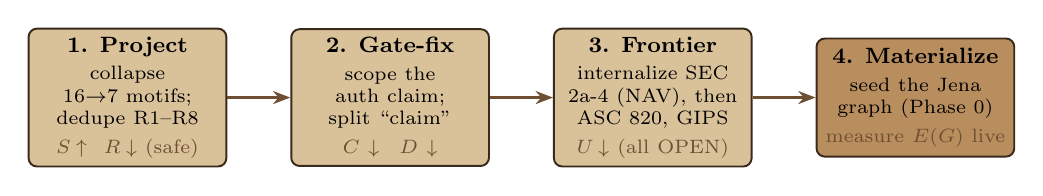
\begin{tikzpicture}[
  font=\footnotesize,
  >={Stealth[length=2.2mm]},
  stage/.style={draw=ratioInk, rounded corners=3pt, align=center,
                text width=23mm, minimum height=15mm, inner sep=3pt, line width=0.7pt},
]
\node[stage, fill=ratioSand] (proj) {\textbf{1. Project}\\[2pt]
  \scriptsize collapse 16$\to$7 motifs; dedupe R1--R8\\[1pt]
  \scriptsize\color{ratioBrown}$S\!\uparrow\ R\!\downarrow$ (safe)};
\node[stage, fill=ratioSand, right=8mm of proj] (gate) {\textbf{2. Gate-fix}\\[2pt]
  \scriptsize scope the auth claim; split ``claim''\\[1pt]
  \scriptsize\color{ratioBrown}$C\!\downarrow\ D\!\downarrow$};
\node[stage, fill=ratioSand, right=8mm of gate] (front) {\textbf{3. Frontier}\\[2pt]
  \scriptsize internalize SEC 2a-4 (NAV), then ASC 820, GIPS\\[1pt]
  \scriptsize\color{ratioBrown}$U\!\downarrow$ (all OPEN)};
\node[stage, fill=ratioTan, right=8mm of front] (mat) {\textbf{4. Materialize}\\[2pt]
  \scriptsize seed the Jena graph (Phase 0)\\[1pt]
  \scriptsize\color{ratioBrown}measure $E(G)$ live};
\draw[->, ratioBrown, line width=1pt] (proj) -- (gate);
\draw[->, ratioBrown, line width=1pt] (gate) -- (front);
\draw[->, ratioBrown, line width=1pt] (front) -- (mat);
\end{tikzpicture}

  \vskip1.0em
  {\footnotesize Each stage moves the energy monotonically --- more $S$/$L$, less $R$/$C$/$D$/$U$ --- the $E(G)$ descent of RFC-001b.}
\end{frame}

% ---------------------------------------------------------------- frame: close
\begin{frame}{The deck is an output of the pipeline}
  \begin{columns}[c]
    \begin{column}{0.6\textwidth}
      \begin{itemize}\setlength\itemsep{4pt}
        \item These graphs are authored as \texttt{.dot} and rendered \textbf{hermetically} (rules\_graphviz $\to$ SVG; tectonic $\to$ deck).
        \item Once Phase 0 materializes the Jena graph, the same figures regenerate from \textbf{SPARQL $\to$ dot}.
        \item So the deck stops being a snapshot someone made --- it becomes the \textbf{crystal photographed each crank}.
        \item Across cranks, watch $E(G)$ descend.
      \end{itemize}
    \end{column}
    \begin{column}{0.38\textwidth}
      \centering
      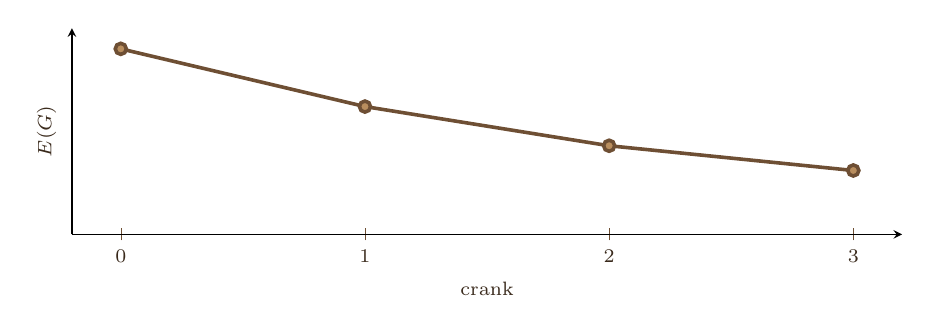
\begin{tikzpicture}
      \begin{axis}[
        width=\linewidth, height=4.2cm,
        xlabel={crank}, ylabel={$E(G)$},
        every axis label/.style={font=\scriptsize\color{ratioInk}},
        xtick={0,1,2,3}, ytick=\empty,
        xmin=-0.2,xmax=3.2, ymin=0, ymax=10,
        axis lines=left, tick style={color=ratioBrown},
        xticklabel style={font=\scriptsize\color{ratioInk}},
      ]
      \addplot[draw=ratioBrown,line width=1.3pt,mark=*,mark options={fill=ratioTan}]
        coordinates {(0,9) (1,6.2) (2,4.3) (3,3.1)};
      \end{axis}
      \end{tikzpicture}\\[2pt]
      {\scriptsize schematic descent; crank-001 is the first point}
    \end{column}
  \end{columns}
\end{frame}

\end{document}
